\documentclass{article}
\usepackage{graphicx}

\title{Triangle Areas}
\author{William Y. Feng}

\begin{document}

\maketitle
``The area of a triangle is half its base times its height." We were taught to memorize this formula in school, but why is it true?

Let's look at a triangle:
\begin{center}
    \centering
    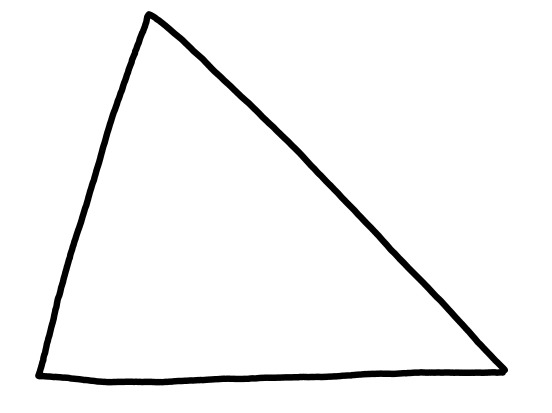
\includegraphics[width=2in]{images/triangle_areas/part_1/raw_triangle.png}
\end{center}
So far, nothing revolutionary. Let's add a box around it:
\begin{center}
    \centering
    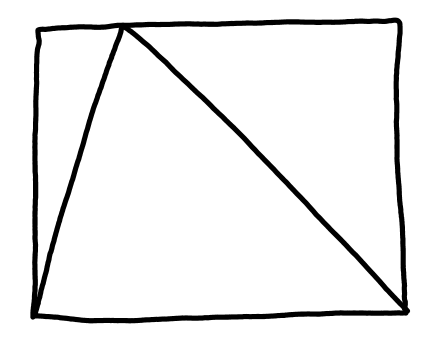
\includegraphics[width=2in]{images/triangle_areas/part_1/triangle_in_box.png}
\end{center}
Still not extremely exciting, but now we can tell that it has a clearly defined base and height, which are the dimensions of its bounding box. The real kicker comes in when we add a \textit{line}:
\begin{center}
    \centering
    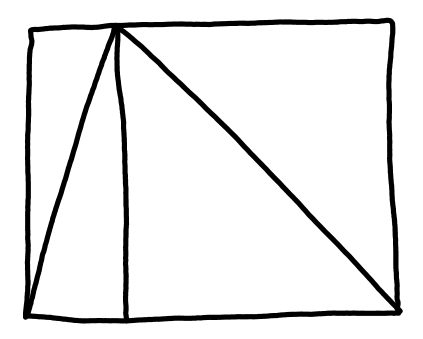
\includegraphics[width=2in]{images/triangle_areas/part_1/triangle_in_box_line.png}
\end{center}
Aha! Now we have two smaller boxes, and the triangle occupies half the area within each box. Therefore, the triangle is half the area of the box, which is its base times its height.

That's pretty neat, you say, but what if we have an obtuse triangle, like the one below? This triangle doesn't lie entirely inside its box, so we can't just draw a line like before to get some witty argument that the triangle's area is half that of the box.
\begin{center}
    \centering
    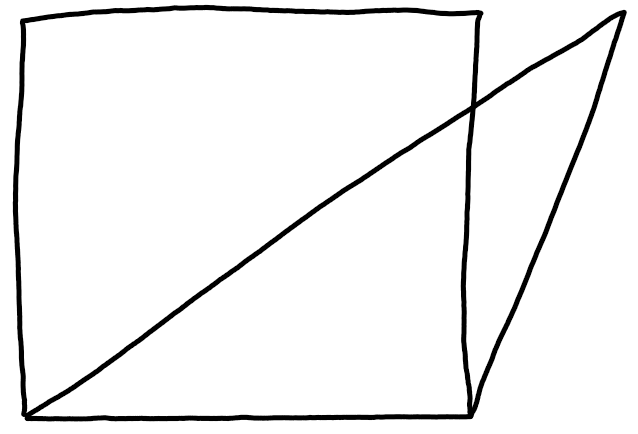
\includegraphics[width=2in]{images/triangle_areas/part_1/obtuse_triangle_in_box.png}
\end{center}
This is true, so let's tilt the box a little so that it becomes a \textbf{parallelogram}:
\begin{center}
    \centering
    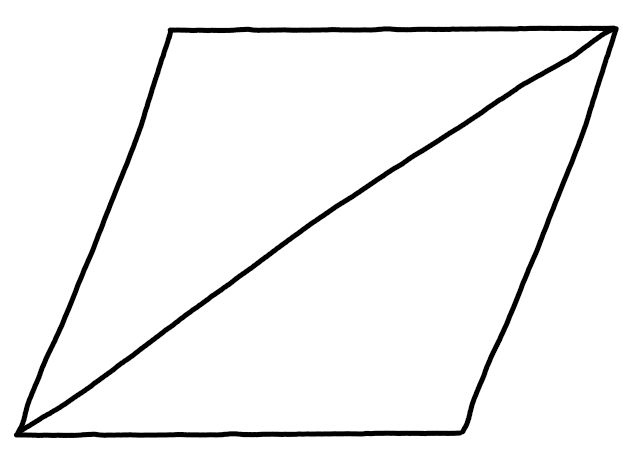
\includegraphics[width=2in]{images/triangle_areas/part_1/obtuse_triangle_in_parallelogram.png}
\end{center}
We see that the area of the triangle is half the area of the parallelogram! Let's remove the triangle from the diagram and add back the box, since we only care about the area of the parallelogram now.
\begin{center}
    \centering
    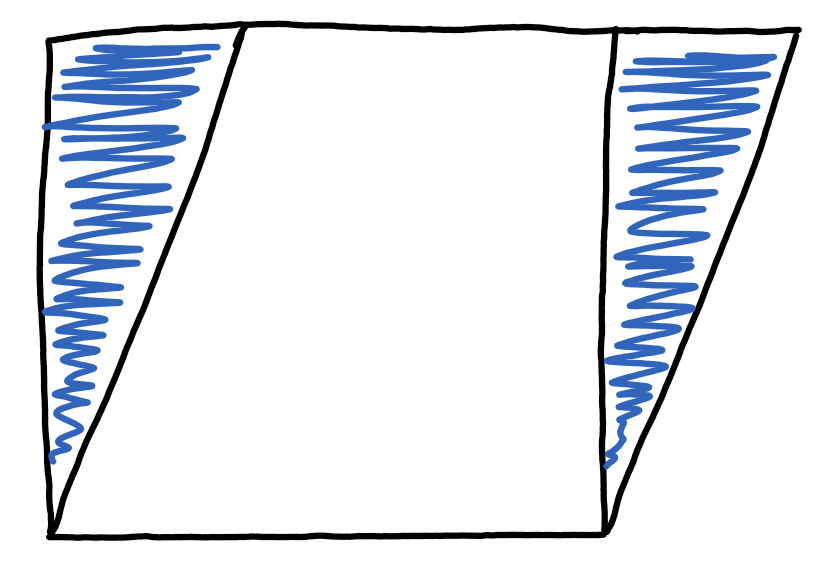
\includegraphics[width=2in]{images/triangle_areas/part_1/parallelogram_box.png}
\end{center}
Those triangular bits have the same area, so the parallelogram actually has the same area as the box. Thus, the area of our original obtuse triangle is still half the area of its box, which is its base times its height.

Now that we have a better idea of why the triangle area formula
\[ A = \frac{bh}{2} \]
is true, let's see one direct application:

\textbf{Triangle area ratios:}

\begin{center}
    \centering
    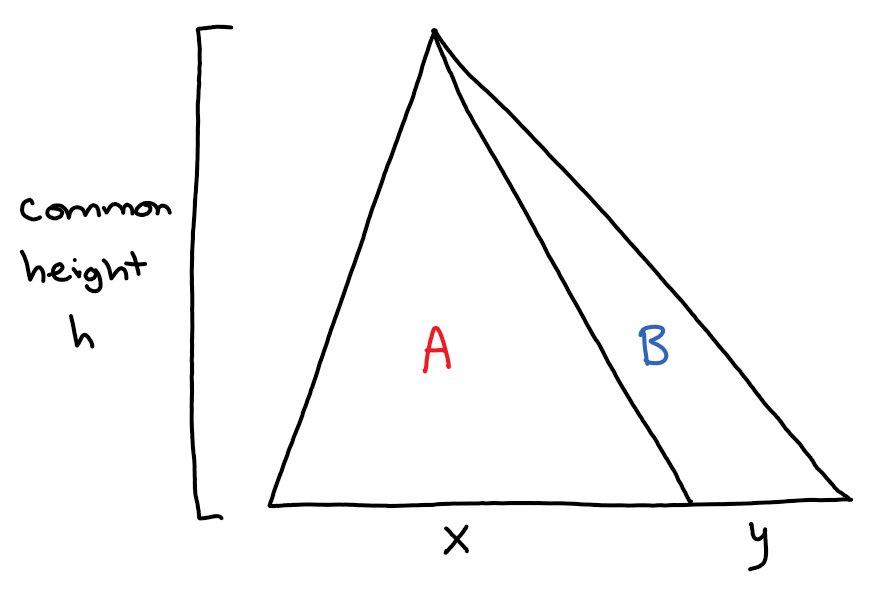
\includegraphics[width=2in]{images/triangle_areas/part_2/common_height.png}
\end{center}

Here we have a big triangle split into two smaller triangles, $A$ and $B$. The two sub-triangles have the same height; let this be $h$.

If $A$'s base has length $x$, then $A$'s area is $(xh)/2$. If $B$'s base has length $y$, then $B$'s area is $(yh)/2$. The \textit{ratio} of these two triangles' areas is thus $x : y$, which gives us the following Very Important Fact: \textbf{if two triangles share the same height, then the ratio of their areas equals the ratio of their bases.}

Let's take a look at one of my favorite examples of this fact in action.

\textbf{Ceva's theorem:}

\begin{center}
    \centering
    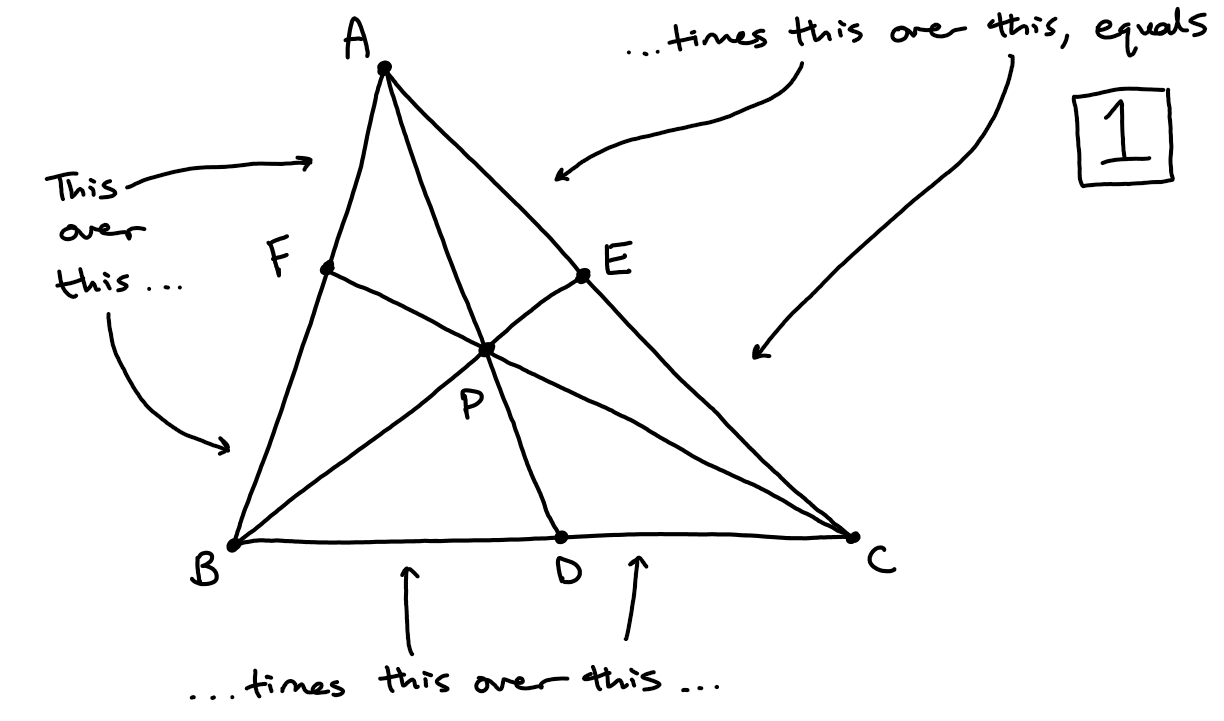
\includegraphics[width=2in]{images/triangle_areas/part_2/ceva_fig0.png}
\end{center}

Let $P$ be a point in the interior of triangle $ABC$. Draw lines from the vertices $A, B, C$ through $P$, and let them hit the opposite sides at $D, E, F$ respectively. \textbf{Ceva's theorem} \footnote{Or at least, one half of it—the full theorem tells us that if the equation holds for arbitrary points $D, E$ and $F$ on the sides of triangle $ABC$, then the lines $AD, BE$, and $CF$ meet at a point $P$.} states that
$$\dfrac{AF}{BF} \cdot \dfrac{BD}{DC} \cdot \dfrac{CE}{AE} = 1.$$
Let's prove it.
\begin{center}
    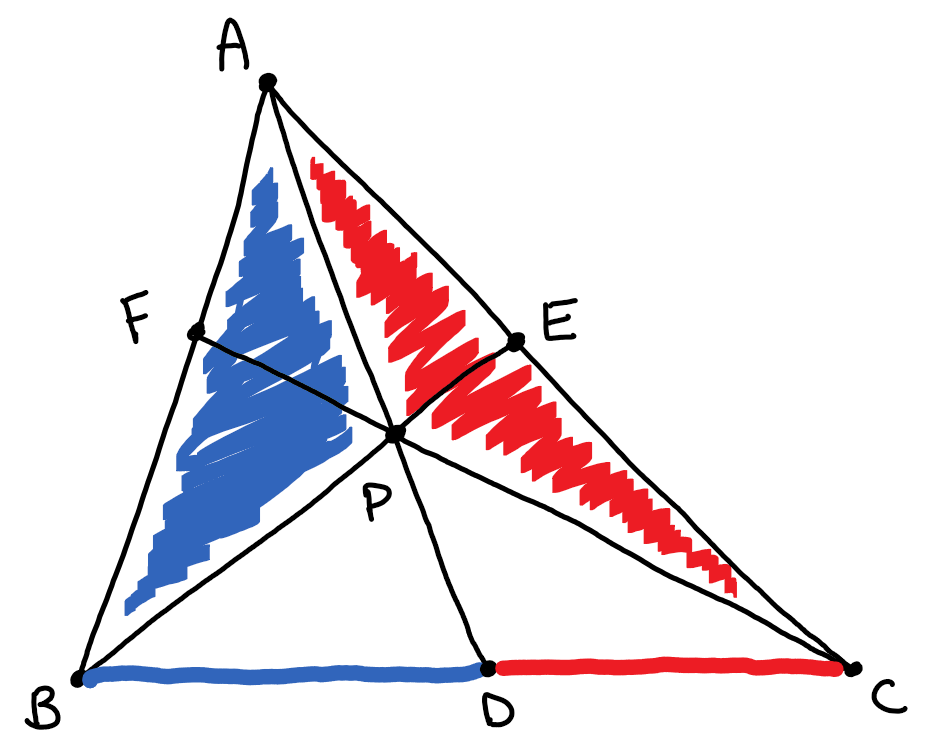
\includegraphics[width=4in]{images/triangle_areas/part_2/ceva_fig1.png}
\end{center}
The key claim is that, in the figure above, the ratio between the blue segment and the red segment ($BD/CD$) equals the ratio between the blue area and the red area ($\triangle ABP$ to $\triangle ACP$). Why is this true?
\begin{enumerate}
    \item We know that the ratio between $BD$ and $CD$ equals the ratio between the areas of triangles $ABD$ and $ACD$, because they share the same height.
    \item The ratio between $BD$ and $CD$ \textit{also} equals the ratio between the areas of triangles $BDP$ and $CDP$.
    \item If we subtract the two triangle ratios, we get exactly what we want!
\end{enumerate}

In other words,
$$\frac{BD}{CD} = \frac{\text{blue area}}{\text{red area}}.$$

Let's color one more triangle, $\triangle BCP$, and let's make it green.
\begin{center}
    \centering
    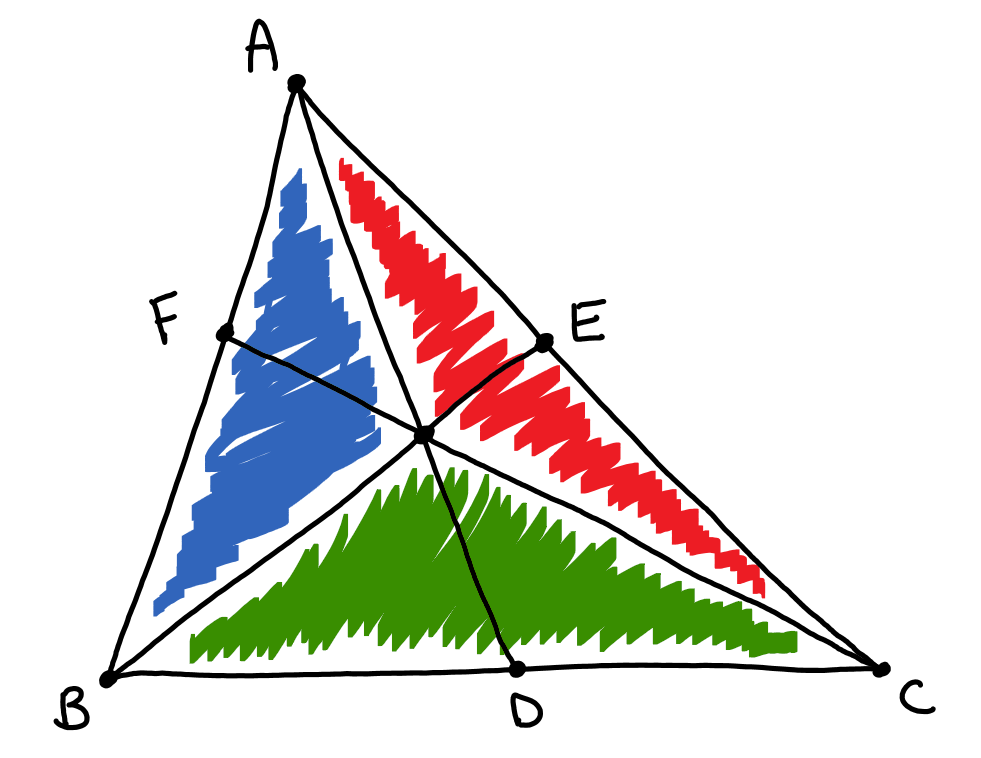
\includegraphics[width=2in]{images/triangle_areas/part_2/ceva_fig2.png}
\end{center}
Applying similar ratio logic as above, we get that
\[\frac{CE}{AE} = \frac{\text{green area}}{\text{red area}}\]
and 
\[\frac{AF}{BF} = \frac{\text{blue area}}{\text{green area}}.\]
So, translating Ceva's theorem, we get that
\[ \dfrac{AF}{FB} \cdot \dfrac{BD}{DC} \cdot \dfrac{CE}{EA} = 1\]
becomes
\[ \frac{\text{blue}}{\text{green}} \cdot \frac{\text{blue}}{\text{red}} \cdot \frac{\text{green}}{\text{red}} = 1. \]
This is obviously true, because everything on top cancels with everything on the bottom. So we're done! We've proved Ceva's theorem, \footnote{one half of it, at least} through the power of triangle areas.
\end{document}